\documentclass[letterpaper]{article}

% NIPS header
\usepackage{nips10submit_e,times} 
\usepackage{helvet} 
\usepackage{courier}
\usepackage{url}

% fancy symbols
\usepackage{amsmath}
\usepackage{amsthm}
\usepackage{amssymb}
% \usepackage{natbib}
\usepackage{graphicx}
\usepackage{subfigure}

\newtheorem{thm}{Theorem}
\newtheorem{lemma}{Lemma}
\newtheorem{definition}{Definition}
\newtheorem{question}{Question}

\title{Learning Review Classification from Different Domains}
\author{Ertan Dogrultan, Cesar Romero, Paul Wais\\
Computer Science Department \\
University of California, Los Angeles\\
Los Angeles, California 90095\\
\texttt{\{ertan,romero\}@cs.ucla.edu, pwais@ucla.edu}}

\nipsfinalcopy

\begin{document}
\maketitle
\begin{abstract}
  In this project, we study the learning task of predicting
  ``usefulness'' votes of product and business reviews.  We have
  obtained 2 million Amazon reviews and 15,000 Yelp reviews annotated
  with voting information.  We wish to predict whether a review will
  achieve a high ranking on the scoreboard of reviews voted
  ``useful''.  In particular, we consider a binary labeling task where
  we assign a positive ``usefulness'' label to a review if its
  positive vote count falls at or above the pth percentile of all vote
  counts (and assign a negative label otherwise).  To predict these
  labels, we have implemented about two dozen textual and contextual
  features inspired by Pang et al. \cite{PangSentimentClassification}
\end{abstract}

\section{Introduction}
\label{sec:introduction}

Review-based social networks empower users to make informed purchasing
decisions.  Amazon and Yelp are two such networks that feature
millions of user-contributed consumer product and local business
reviews.  A central challenge facing these networks is the task of
quickly connecting users with useful review content.  For example,
many products and businesses on these websites feature hundreds of
user-contributed reviews, so the site must automatically identify and
spotlight the most relevant of these reviews in order to keep viewers
engaged.  In order to surface the best content, many review-based
social networks employ a user voting mechanism that enables viewers to
anonymously vote a review as ``useful.''  Unfortunately, though many
viewers do make use of this feature, most reviews do not receive votes
(see Figure \ref{fig:vote-histos}).  In this work, we study applying modern
machine learning algorithms to textual review features in order to
automatically predict if a review will receive ``useful'' votes.

An additional problem facing these networks is to spotlight quality
content in emerging areas of the site.  For example, when a social
network extends to a new foreign language or expands to a new product
domain, the network might purchase or otherwise establish seed review
content, but these reviews will not feature viewer-contributed votes.
In this setting, it is useful to adapt a model trained on existing
user votes to spotlight new content that viewers will find useful.  In
this work, we study how to fulfill this task using a domain adaptation
technique \cite{JennLearnDiffDomains}.

The remainder of this paper proceeds as follows: first we describe the novel 
features we use and contrast them with related work in sentiment 
classification.  Next, we present the results of applying traditional 
supervised learning algorithms to learn to predict the ``usefullness'' of 
reviews from Amazon and Yelp.  Next, we investigate the problem of domain 
adaptation by training a linear SVM on a preponderance of Amazon review data 
and a small sample data.  Despite spending considerable effort on feature 
engineering and classifier tuning, we observe high error rates for both of the 
aforementioned experiments.  We find that the problem of predicting usefulness 
is harder than the related problem of sentiment classification.  We conclude 
with suggestions for additional features and experiments that may result in a more accurate model.

\begin{figure}[h]
    \label{fig:vote-histos}
	\centering
	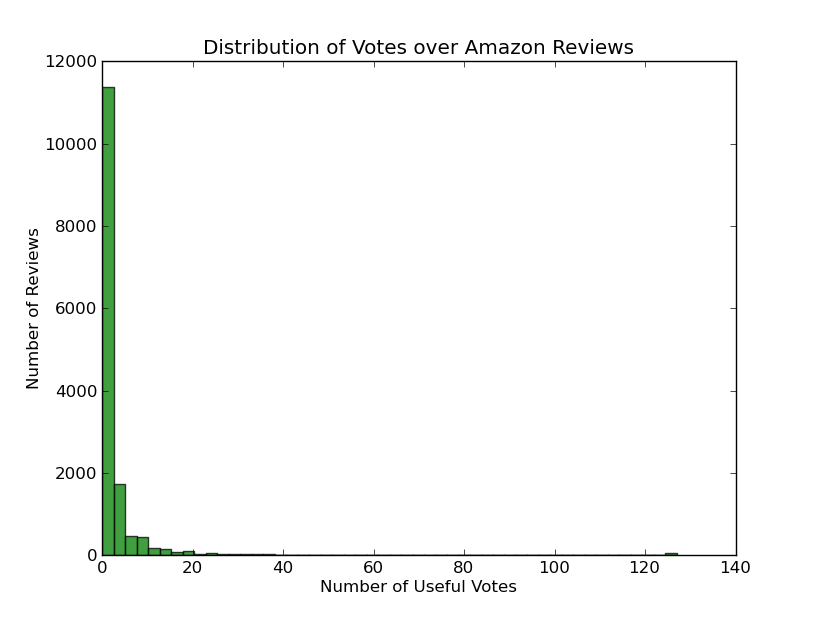
\includegraphics[width=0.30\linewidth]{amz_histo}
    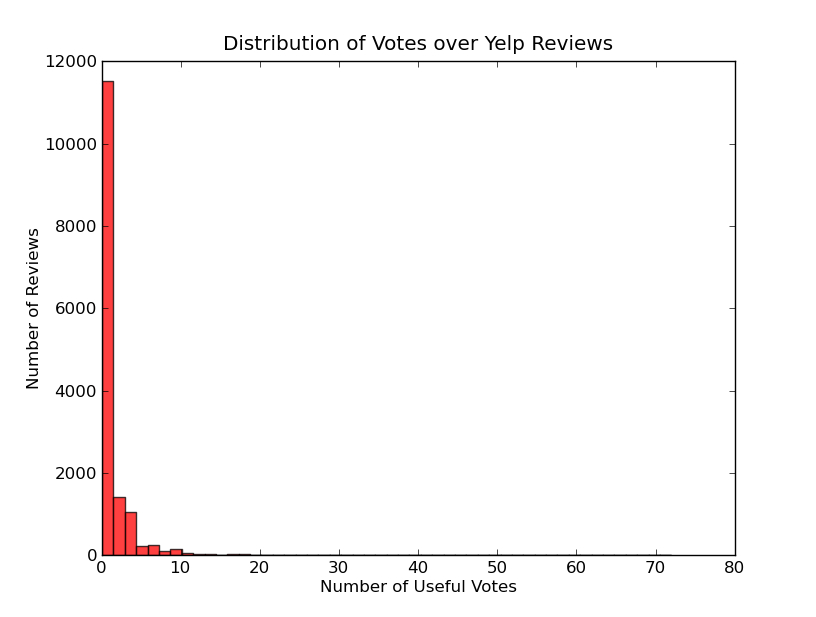
\includegraphics[width=0.30\linewidth]{yelp_histo}
	\caption{Histograms of votes in samples of 15,000 Amazon and Yelp reviews.
    Most reviews have zero votes.}
\end{figure}

\section{Setting and Related Work}
Our approach builds on related work in sentiment classification that seeks to use 
review text to predict the ratings of users' reviews.  Pang et al \cite{PangSentimentClassification}
apply several supervised machine learning algorithms to product reviews and observe that 
standard, untuned algorithms are capable of approximately $85\%$ accuracy.  They hypothesize that
a small set of words decide sentiment and encode input text in attemp to learn these words. 
Their model represents reviews as sparse vectors in a high-dimensional space where the $i$th component 
of a vector $\vec{x}$ indciates the count or presence for a single unigram or bigram.  They observe
that SVMs peform slightly better when trained on vectors of word presence rather than counts.

Dodds et al \cite{DoddsANEWPaper} have conducted a related study and build upon work in 
pyscholinguistics towards building a ``hedonometer'' capable of predicting positive 
and negative sentiment from unlabeled text.  Their work devises a simple model utilizing the 
valence scores of words from the ANEW data set

\section{Feature Extraction and Labeling the Data}
We have divided the features into several categories.
\subsection{Word Frequencies and Counts}
Our simplest feature is the number of words in the review. Similarly,
we calculate the average number of words per sentence and total number
of sentences in the review. Additionally, we count the number of URLs.

We obtain many different sets of words with respect to their
contextual meanings (i.g. time, space, comparison, contrast, summary,
suggestion, emphasis) and we count the number of occurrences of these
in a review. For instance, comparison words are \emph{similarly,
  likewise,} etc., contrast words are \emph{but, however,
  nevertheless, in spite of,} etc. Moreover, we have some other sets
of special words such as SAT, GRE lists on which we apply the same
procedure.  We normalize by dividing each of them by the total number
of words in the body of the review and use them as features.

\subsection{Sentential Errors}
We count the grammar and spelling errors with libraries using
Microsoft Word. We also consider the number of capitalization
mistakes and words with all capital letters. Like before, we divide
these counts by the total number of words in the review.

\subsection{Scores}
ANEW~\cite{DoddsANEWPaper}.

\subsection{Product/Service Related Features} 
This feature is somewhat different than the previous ones; it depends
on the product as opposed to a particular review. We include the price
of the product from the Amazon data set and discretize it so that we
have a corresponding measurement of price range as we have in Yelp
reviews (i.e. an integer between 1 (cheap) and 4 (expensive)).

\subsection{Deciding on the Labeling}
In the early experiments, we used $50^{th}$ percentile cutoff to label
the review as useful. In other words, if the nuimber of positive votes
for a review is above the $50^{th}$ percentile, we labeled it as
useful. This approach affected our classification accuracy negatively,
and we decided to try to eliminate some noise from the data by pushing
the thresholds to more extreme values. Currently, we label a review as
useful if its positive count is in the $75^{th}$ percentile or above
and not useful if they are in the $5^{th}$ percentile or below. We
observe the reflection of this approach on the confusion matrices. We
will discuss more about this in Section \ref{sec:single_domain}.

\section{Single Domain Experiments}
\label{sec:single_domain}  
We run the experiments using the open-source data mining software
WEKA~\cite{weka}, and present the results for three algorithms:
Support Vector Machines, Adaboost and Naive Bayes with two different
feature encodings.

In the first encoding, we have different sets of words as we described
in Section~\ref{sec:features}. We compute the frequencies of those
words and use each calculated frequency as a single feature. We refer to
this encoding as \emph{dense}.

Our second feature encoding aims to generate more weak classifiers out
of the sets of words. We assume every word from these sets is a
feature, and we get the corresponding weak classifier by computing
their frequencies. We refer to this encoding as \emph{sparse}. The
main motivation behind the sparse features is increasing the dimension
for classification. This can be useful for SVMs and Adaboost
algorithms.

\begin{table}[ht]
\centering
\begin{tabular}{c | c c | c c}
 & \multicolumn{2}{|c|}{Amazon} & \multicolumn{2}{|c}{Yelp} \\
\hline
Algorithm & Training Err. & Cross Val.(5 fold) & Training Err. & Cross Val.(5 fold)\\
\hline
SVM (Linear) 		& $71.0316\%$ & $70.8\%$ & $70.305\%$ & $70.2879\%$\\
SVM (Polynomial) 	& $73.1041\%$ & $72.4316\%$ & --- & $71.3417\%$\\
SVM (Gaussian) 		& $66.053\%$ & $66.053\%$ & $68.7971\%$ & $69.1484\%$\\
AdaBoost 			& $71.0316\%$ & $72.201\%$ & $71.3588\%$ & $70.3136\%$\\ 
Naive Bayes 		& $70.719\%$ & $70.6727\%$ & $66.9037\%$ & $66.5781\%$\\ 
\end{tabular}
\caption{Accuracy using dense feature encoding}
\label{tab:dense}
\end{table}


\begin{table}[ht]
\centering
\begin{tabular}{c | c c | c c}
 & \multicolumn{2}{|c|}{Amazon} & \multicolumn{2}{|c}{Yelp} \\
\hline
Algorithm & Training Err. & Cross Val.(5 fold) & Training Err. & Cross Val.(5 fold)\\
\hline
SVM (Linear) 		& --- & $72.2357\%$ 		& --- & $70.0163\%$\\
SVM (Polynomial) 	& --- & $66.053\%$ 		& --- & $70.0592\%$\\
SVM (Gaussian) 		& --- & $72.4673\%$ 		& --- & $71.1062\%$\\
AdaBoost 			& $71.68\%$   & $70.7769\%$ & $71.2091\%$ & $70.7286\%$\\ 
Naive Bayes 		& $76.8091\%$ & $73.0346\%$ & $77.1733\%$ & $67.9567\%$\\ 
\end{tabular}
\caption{Accuracy using sparse feature encoding}
\label{tab:sparse}
\end{table}

Tables~\ref{tab:dense} and~\ref{tab:sparse} show the results for this
set of experiments. First, we want to focuson the performance
improvement Naive Bayes shows when switching to sparse encoding. We
said in the progress report that the main problem with this classifier
is believed to be the lack of low entropy feature
distributions~\cite{naivebayes}. We pointed out that the unrealistic
assumption of conditional independence between the features hurts the
classification significantly; this is precisely the nature of the
dense feature encoding. One thing to note is that there are overlaps
amongst the word lists mentioned before; not only in the actual words
but in meaning as well. Therefore, switching to sparse encoding
removes dependecies between features that could normally reduce the
performance of Naive Bayes. The Tables show how the accuracy increases
from $70\%$ to $76\%$ for Amazon and from $66\%$ to $77\%$ for Yelp.

In many applications, Adaboost algorithm tends to have low training
error, so we investigate the performance of Adaboost more closely. We
look at our weak classifiers and the corresponding errors,
$\epsilon_t$. At each step, the weak classifier, $h_t(x)$, having the
minimum error on the weighted samples is chosen greedily. The first
chosen weak classifier (which is usually the number of words in the
text with a certain threshold) has $\epsilon_t \approx 0.34$. However,
latter classifiers have very high error rates, $\epsilon_t \approx
0.4999999$ which can be considered random decision in practice. As we
looked at the histograms of feature distributions over the labeled
samples, we observed that they were either very sparse (i.e. few
buckets have reviews in them) or the histograms overlapped. As we
extract a weak classifier that corresponds to a feature, the threshold
cannot classify significantly better than random decision due to this
overlap. Keeping this empirical observation in mind, we revisit the
upper bound for the training error for
Adaboost~\cite{adaboost,adaboost2}. We have
\[
err(H) \leq e^{-2\gamma^2 T}
\]
where $\forall t$, $\gamma_t \geq \gamma $ and $\gamma > 0$. In our
experiments, we witness an arbitrarily small $\gamma$. We believe that
this explains the poor performance of the strong classifier.

Looking at the performance of Adaboost and linear SVMs with dense and
sparse encodings, we observe similar accuracies for both Amazon and
Yelp data. We believe that the class distribution (the choice of
percentile to label the sample as useful) has a significant effect on
the accuracy. This conclusion originates from the observation of
``bad'' confusion matrices ($CM$) for the classifiers. Indeed, as we
look at the confusion matrices of both algorithms on the Amazon data
set in Equation~\ref{eq:confusion}, we do not see the desired dominant
diagonal.
\begin{equation}
\label{eq:confusion}
CM_{Adaboost} = \left(
\begin{matrix}
4551 & 1154\\
1247 & 1685
\end{matrix}
\right)
\qquad
CM_{linearSVM} = \left(
\begin{matrix}
5486 & 219\\
2303 & 629
\end{matrix}
\right)
\end{equation}
As we investigate further by changing the labeling method
for the reviews, we see the effect of class distributions directly on
the confusion matrices. An interesting perspective to compare the
behavior of Adaboost and linear SVM might be looking at the specific
examples represented in these confusion matrices instead of the training
accuracy. As you can see in (\ref{eq:confusion}), Adaboost is in much
better condition than linear SVMs in this aspect. However, we believe
we need to do a literature survey to have a better method and a more
rigorous explanation
for this comparison, so we leave this task as a future work.

\section{Domain Adaptation}
\label{sec:background}

We are interested in being able to classify reviews in general - not
just from a specific source or category. This would allow for reviews
to be classified automatically even on domains where the amount of
labeled data is very limited. This problem has been studied recently
as \emph{domain adaptation}~\cite{JennLearnDiffDomains}. In this
problem, there is a source domain $S$ and a target domain $T$. The
goal is to be able to classify reviews in $T$ when most of our data
comes from $S$. To be able to estimate a bound on the error, two
important concepts are taken into account: the divergence between
unlabeled data in both domains and the combined empirical error.

In this setting, a classifier-induced divergence
suffices~\cite{JennLearnDiffDomains}. It is obtained by training a
linear classifier to learn to which domain a review belongs to. The
error of this classifier is used to estimate the divergence we are
interested in.

Given the two domains we are interesting in learning a hypothesis $h$
that minimizes an empirical error that combines both domains. This is
precisely the $\alpha$-error defined as $\alpha \hat
\epsilon_T(h)+(1-\alpha)\hat \epsilon_S(h)$, where $\hat \epsilon_S$
and $\hat \epsilon_T$ are the source and target errors
respectively~\cite{JennLearnDiffDomains}.

With this ingredients, an approximation to the bound is given by
Equation~(\ref{eq:alphaerror}). Where $\zeta(U_S,U_T)$ is the
empirical divergence and $\beta$ is the fraction of examples that come
from the target domain.

\begin{equation}
  \label{eq:alphaerror}
  f(\alpha)=\sqrt{\frac{C}{m}\left(\frac{\alpha^2}{\beta} + \frac{(1-\alpha)^2}{1-\beta}\right)}+(1-\alpha)\zeta(U_S,U_T)
\end{equation}

\begin{figure*}[h]
	\centering
	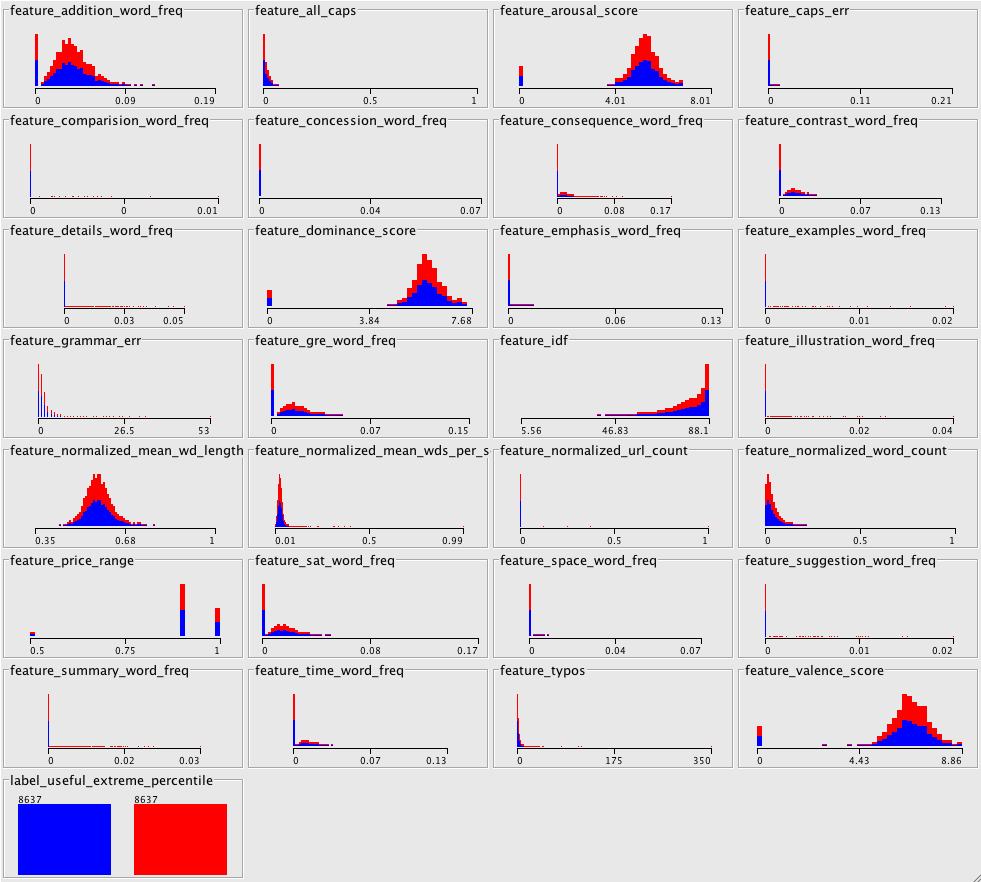
\includegraphics[width=0.75\linewidth]{adaptation_unlabeled_features}
	\caption{Feature distributions for the unlabeled data sets $U_{\textrm{A}}$ and $U_{\textrm{Y}}$.  
	Blue indicates Amazon data feature values and red indicates Yelp feature values.}
\end{figure*}

\subsection{Experiments}
\label{sec:domain-adaptation}

In this set of experiments we use Support Vector Machines to learn
from a combination of both domains; Yelp is considered to be the
\emph{target domain} and Amazon the \emph{source domain}.

We estimate the divergence $\zeta(U_S,U_T)$ as described in the
previous section combining 15,000 examples from each domain.

We performed two sets of experiments. First, we fix the number of
examples from the source domain constant $m_s=2500$, and we vary the
examples from the target distribution $m_t \in \{250, 500, 1000,
2000\}$. Then, we fix $m_t=2500$ constant and we vary $m_s$ in the
same way. 

Figure~\ref{fig:domain-adaptation} shows the results of both
experiments. The left column corresponds to the first experiments where
$m_S$ is fixed; the right column to the experiments where $m_T$ is
fixed. Top row shows a theoretical bound on the error given by
Equation~(\ref{eq:alphaerror}) and the bottom row shows experimental
results.

\begin{figure}
  \centering
  \subfigure[$\zeta(U_S, U_T)=1, m_S=2500$]
  {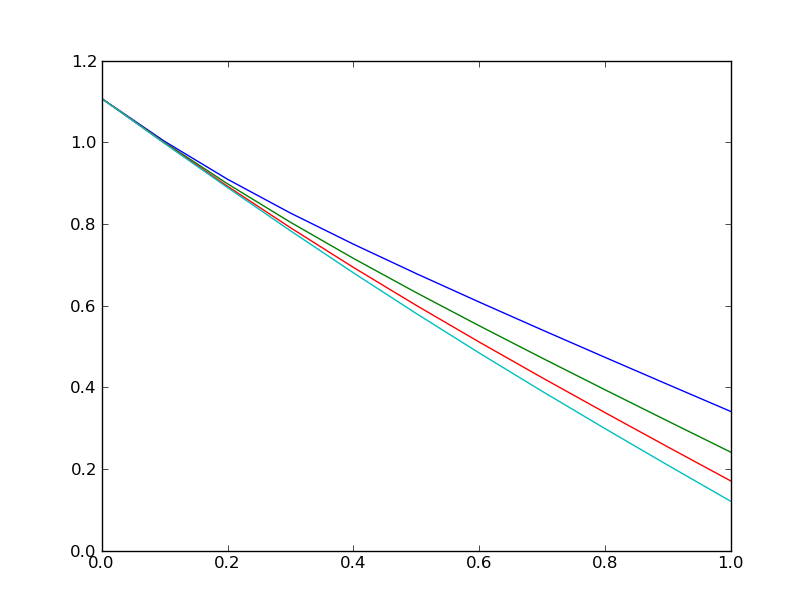
\includegraphics[scale=.3]{adaptation_bound_1_S}}
  \subfigure[$\zeta(U_S, U_T)=1, m_T=2500$]
  {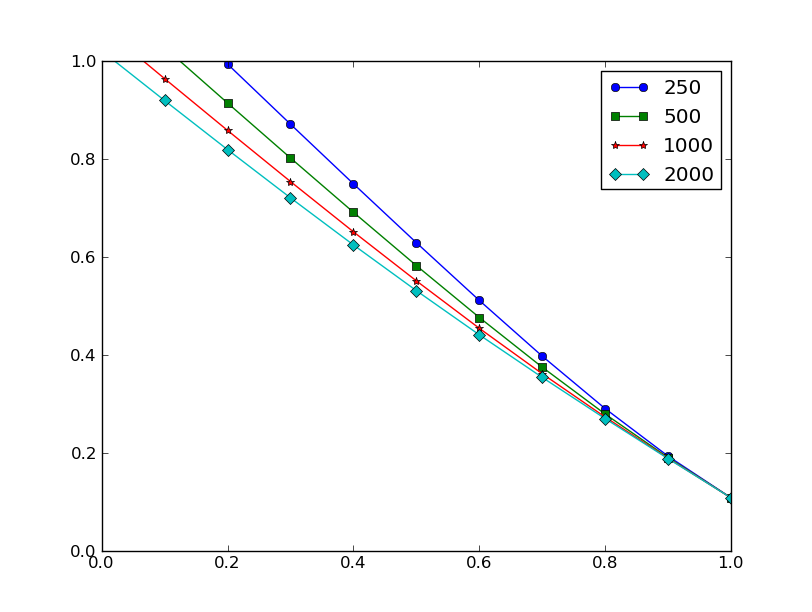
\includegraphics[scale=.3]{adaptation_bound_1_T}}
  \subfigure%[$\zeta(U_S, U_T)=1, m_S=2500$]
  {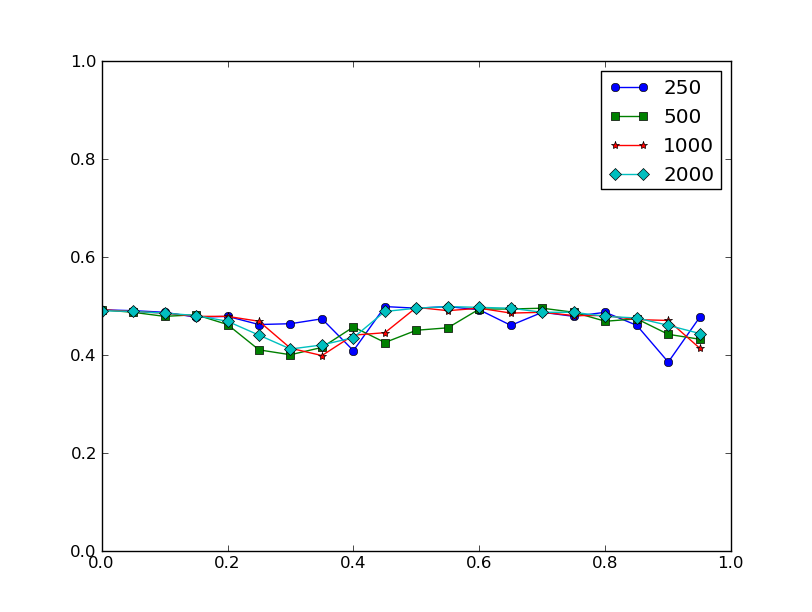
\includegraphics[scale=.3]{adaptation_err_S}}
  \subfigure%[$\zeta(U_S, U_T)=1, m_T=2500$]
  {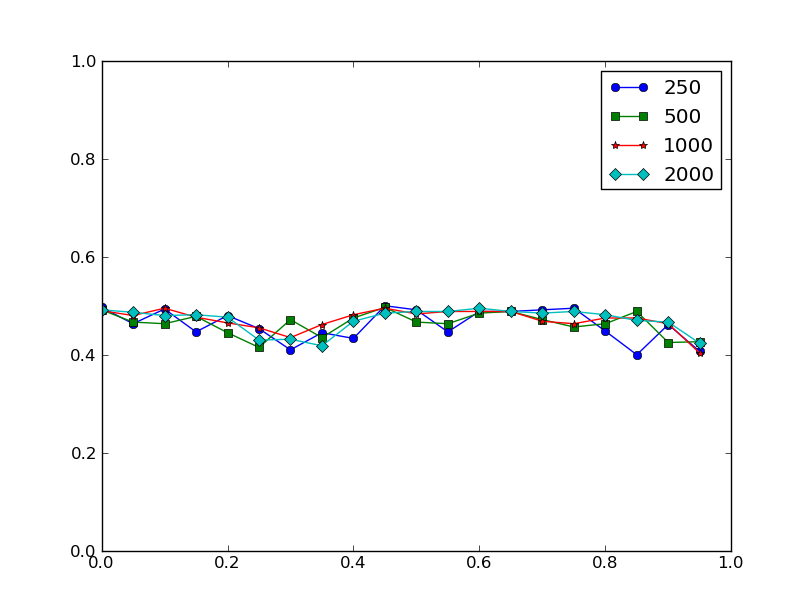
\includegraphics[scale=.3]{adaptation_err_T}}
  \caption{Domain adaptation experiments. The $\alpha$-error is shown as a function of $\alpha$ for different combinations of source and target examples.}
  \label{fig:domain-adaptation}
\end{figure}

\section{Future work}
\label{sec:future-work}

Looking at the performances of the algorithms, we observe Adaboost and
linear SVM have similar accuracies on most of the various experiment
instances. As stated in Section \ref{sec:single_domain} one of the
obvious differences is the quality of the confusion matrices. We would
like to investigate the incorrectly classified examples for each
algorithm and come up with an explanation related to what it is
minimizing for classification.  Furthermore, we would like to give a
more rigorous explanation on why Naive Bayes classifier has a
dominating accuracy in sparse feature encoding by comparing the
objective functions of our algorithms.

For domain adaptation part, we would like to see how well the
classifier performs when the distance between the target and source
distribution varies keeping the $\beta$ fixed. To alter $\zeta$, we
can consider only a specific category on each domain.

For example, from the source domain (Amazon), we could consider the
set of categories $C_S$=\{ Books, Electronics, DVDs and Clothing\};
from the target domain (Yelp), we could consider category
$C_T=$\{Restaurants\}. For each combination in $C_s\times C_T$ we
train and test a different linear classifier to estimate the distance
between the two distributions of each configuration.

\section{Conclusion}
\label{sec:conclusion}

We have used different machine learning algorithms to determine the
quality of a review using real data from Amazon and Yelp. We have
approached this task as a domain adaptation problem. In particular, we
tried to use a large set of Amazon reviews to predict the quality of
Yelp reviews. One of the most important remarks is the effect of noise
in the data and choice of the right features for classification. We
believe feature extraction per se can be the most significant factor
for the accuracy of the classification. Unfortunately, we have
approached this problem using just intuition rather than a data driven
model or following previous work.  We believe its impact on the domain
adaptation experiments is not negligible. On the other hand, this has
not affected the goal of this project; we have aimed to look at the
nature of the algorithms and the domain adaptation
problem. However, we believe its impact on the domain adaptation
experiments is not negligible. 


\bibliographystyle{IEEEtran}
\bibliography{bib,IEEEabrv}

\end{document}
